% Options for packages loaded elsewhere
\PassOptionsToPackage{unicode}{hyperref}
\PassOptionsToPackage{hyphens}{url}
\PassOptionsToPackage{dvipsnames,svgnames,x11names}{xcolor}
%
\documentclass[
]{article}

\usepackage{amsmath,amssymb}
\usepackage{iftex}
\ifPDFTeX
  \usepackage[T1]{fontenc}
  \usepackage[utf8]{inputenc}
  \usepackage{textcomp} % provide euro and other symbols
\else % if luatex or xetex
  \usepackage{unicode-math}
  \defaultfontfeatures{Scale=MatchLowercase}
  \defaultfontfeatures[\rmfamily]{Ligatures=TeX,Scale=1}
\fi
\usepackage{lmodern}
\ifPDFTeX\else  
    % xetex/luatex font selection
\fi
% Use upquote if available, for straight quotes in verbatim environments
\IfFileExists{upquote.sty}{\usepackage{upquote}}{}
\IfFileExists{microtype.sty}{% use microtype if available
  \usepackage[]{microtype}
  \UseMicrotypeSet[protrusion]{basicmath} % disable protrusion for tt fonts
}{}
\makeatletter
\@ifundefined{KOMAClassName}{% if non-KOMA class
  \IfFileExists{parskip.sty}{%
    \usepackage{parskip}
  }{% else
    \setlength{\parindent}{0pt}
    \setlength{\parskip}{6pt plus 2pt minus 1pt}}
}{% if KOMA class
  \KOMAoptions{parskip=half}}
\makeatother
\usepackage{xcolor}
\setlength{\emergencystretch}{3em} % prevent overfull lines
\setcounter{secnumdepth}{-\maxdimen} % remove section numbering
% Make \paragraph and \subparagraph free-standing
\makeatletter
\ifx\paragraph\undefined\else
  \let\oldparagraph\paragraph
  \renewcommand{\paragraph}{
    \@ifstar
      \xxxParagraphStar
      \xxxParagraphNoStar
  }
  \newcommand{\xxxParagraphStar}[1]{\oldparagraph*{#1}\mbox{}}
  \newcommand{\xxxParagraphNoStar}[1]{\oldparagraph{#1}\mbox{}}
\fi
\ifx\subparagraph\undefined\else
  \let\oldsubparagraph\subparagraph
  \renewcommand{\subparagraph}{
    \@ifstar
      \xxxSubParagraphStar
      \xxxSubParagraphNoStar
  }
  \newcommand{\xxxSubParagraphStar}[1]{\oldsubparagraph*{#1}\mbox{}}
  \newcommand{\xxxSubParagraphNoStar}[1]{\oldsubparagraph{#1}\mbox{}}
\fi
\makeatother


\providecommand{\tightlist}{%
  \setlength{\itemsep}{0pt}\setlength{\parskip}{0pt}}\usepackage{longtable,booktabs,array}
\usepackage{calc} % for calculating minipage widths
% Correct order of tables after \paragraph or \subparagraph
\usepackage{etoolbox}
\makeatletter
\patchcmd\longtable{\par}{\if@noskipsec\mbox{}\fi\par}{}{}
\makeatother
% Allow footnotes in longtable head/foot
\IfFileExists{footnotehyper.sty}{\usepackage{footnotehyper}}{\usepackage{footnote}}
\makesavenoteenv{longtable}
\usepackage{graphicx}
\makeatletter
\def\maxwidth{\ifdim\Gin@nat@width>\linewidth\linewidth\else\Gin@nat@width\fi}
\def\maxheight{\ifdim\Gin@nat@height>\textheight\textheight\else\Gin@nat@height\fi}
\makeatother
% Scale images if necessary, so that they will not overflow the page
% margins by default, and it is still possible to overwrite the defaults
% using explicit options in \includegraphics[width, height, ...]{}
\setkeys{Gin}{width=\maxwidth,height=\maxheight,keepaspectratio}
% Set default figure placement to htbp
\makeatletter
\def\fps@figure{htbp}
\makeatother
% definitions for citeproc citations
\NewDocumentCommand\citeproctext{}{}
\NewDocumentCommand\citeproc{mm}{%
  \begingroup\def\citeproctext{#2}\cite{#1}\endgroup}
\makeatletter
 % allow citations to break across lines
 \let\@cite@ofmt\@firstofone
 % avoid brackets around text for \cite:
 \def\@biblabel#1{}
 \def\@cite#1#2{{#1\if@tempswa , #2\fi}}
\makeatother
\newlength{\cslhangindent}
\setlength{\cslhangindent}{1.5em}
\newlength{\csllabelwidth}
\setlength{\csllabelwidth}{3em}
\newenvironment{CSLReferences}[2] % #1 hanging-indent, #2 entry-spacing
 {\begin{list}{}{%
  \setlength{\itemindent}{0pt}
  \setlength{\leftmargin}{0pt}
  \setlength{\parsep}{0pt}
  % turn on hanging indent if param 1 is 1
  \ifodd #1
   \setlength{\leftmargin}{\cslhangindent}
   \setlength{\itemindent}{-1\cslhangindent}
  \fi
  % set entry spacing
  \setlength{\itemsep}{#2\baselineskip}}}
 {\end{list}}
\usepackage{calc}
\newcommand{\CSLBlock}[1]{\hfill\break\parbox[t]{\linewidth}{\strut\ignorespaces#1\strut}}
\newcommand{\CSLLeftMargin}[1]{\parbox[t]{\csllabelwidth}{\strut#1\strut}}
\newcommand{\CSLRightInline}[1]{\parbox[t]{\linewidth - \csllabelwidth}{\strut#1\strut}}
\newcommand{\CSLIndent}[1]{\hspace{\cslhangindent}#1}

\usepackage{fancyhdr} % Load the fancyhdr package
\pagestyle{fancy} % Enable fancy page style
\fancyhf{} % Clear all default header/footer settings
\fancyhead[R]{\thepage} % Add page numbers to the top-right corner
\renewcommand{\headrulewidth}{0pt} % Remove the horizontal line in the header
\renewcommand{\footrulewidth}{0pt} % Remove the horizontal line in the footer
\makeatletter
\@ifpackageloaded{caption}{}{\usepackage{caption}}
\AtBeginDocument{%
\ifdefined\contentsname
  \renewcommand*\contentsname{Table of contents}
\else
  \newcommand\contentsname{Table of contents}
\fi
\ifdefined\listfigurename
  \renewcommand*\listfigurename{List of Figures}
\else
  \newcommand\listfigurename{List of Figures}
\fi
\ifdefined\listtablename
  \renewcommand*\listtablename{List of Tables}
\else
  \newcommand\listtablename{List of Tables}
\fi
\ifdefined\figurename
  \renewcommand*\figurename{Figure}
\else
  \newcommand\figurename{Figure}
\fi
\ifdefined\tablename
  \renewcommand*\tablename{Table}
\else
  \newcommand\tablename{Table}
\fi
}
\@ifpackageloaded{float}{}{\usepackage{float}}
\floatstyle{ruled}
\@ifundefined{c@chapter}{\newfloat{codelisting}{h}{lop}}{\newfloat{codelisting}{h}{lop}[chapter]}
\floatname{codelisting}{Listing}
\newcommand*\listoflistings{\listof{codelisting}{List of Listings}}
\makeatother
\makeatletter
\makeatother
\makeatletter
\@ifpackageloaded{caption}{}{\usepackage{caption}}
\@ifpackageloaded{subcaption}{}{\usepackage{subcaption}}
\makeatother

\ifLuaTeX
  \usepackage{selnolig}  % disable illegal ligatures
\fi
\usepackage{bookmark}

\IfFileExists{xurl.sty}{\usepackage{xurl}}{} % add URL line breaks if available
\urlstyle{same} % disable monospaced font for URLs
\hypersetup{
  pdftitle={Team Assignment - Team 4},
  colorlinks=true,
  linkcolor={blue},
  filecolor={Maroon},
  citecolor={Blue},
  urlcolor={Blue},
  pdfcreator={LaTeX via pandoc}}


\title{Team Assignment - Team 4}
\author{Hanuye Wang (2129151), Shaghi Sharifian (2123294), Timo
Timmermans (2052302), Vietlinh Pham (2148460), Patryk Slomka (2049498)}
\date{2024-12-14}

\begin{document}
\maketitle

\renewcommand*\contentsname{Table of contents}
{
\hypersetup{linkcolor=}
\setcounter{tocdepth}{3}
\tableofcontents
}

\section{Executive Summary}\label{executive-summary}

The research addresses the dynamics and connections between Mexican
cartels using Exponential Graph Models (ERGMs). The main focus is set
upon the rivalries between the cartels and what are the main reasons for
them to form. Our study explicitly addresses three research questions:

\begin{enumerate}
\def\labelenumi{\arabic{enumi}.}
\tightlist
\item
  Do cartels with a common enemy avoid rivalry between each other?
\item
  Are cartels with higher centrality more likely to engage in conflicts
  with other cartels?
\item
  How do geographic territories of operation affect rivalry formation?
\end{enumerate}

The above-mentioned re search questions propose the ideas that shared
enemy of two cartels lead to no rivalry between those two parties;
higher centrality of the cartel node increases the probability of
conflict with other cartels; geographic factors like area of operation
play a crucial role in creation of rivalries. Our results show the law
enforcement and policymakers that cartels with shared enemy are less
likely to be enemies, the geographic location of the cartel increases
the likelihood of having rivals, and that the centrality of the cartel
in alliance network not necessarily lead to having more rivals in the
network.

\section{Introduction}\label{introduction}

The Mexican cartels have long been notorious for their effectiveness and
power, employing approximately 175,000 individuals (Smith (2021)) and
being responsible for 14,000 homicides in 2022 (Uppsala Conflict Data
Program (2022)). Currently, Mexico's illicit networks are once again
characterized by a bipolar cartel structure. While this bipolarity was
once dominated by the Sinaloa Cartel and Los Zetas in the 2000s (Staff
(n.d.)), today the two primary poles of power are the Sinaloa Cartel and
the Cártel de Jalisco Nueva Generación (CJNG). However, they do not
operate in isolation; numerous smaller cartels and criminal groups also
influence Mexico's illicit industries and have the potential to rise to
prominence under favorable conditions, as has repeatedly occurred
throughout the past century (Jones et al. (2022)).

The potential collapse of CJNG leadership through death or arrest or
further fragmentation within the Sinaloa Cartel due to internal
conflicts raises critical questions about which organizations may emerge
to fill the power vacuum. Understanding these dynamics is therefore
essential to proactively identify new threats. Not only is this
important for policymakers in Mexico and the United States but also for
those in Europe, particularly the Netherlands, as both of Mexico's major
cartels are expanding their operations globally, establishing drug
production facilities and distribution networks with the assistance of
local criminal organizations (Europol-DEA et al. (n.d.)).

To address these questions, it is important to analyze how both
endogenous and exogenous factors influence cartel rivalries and,
consequently, their power within the illicit industry. Earlier research
has been done on the alliances and rivalries between the cartels. For
example, by Jones et al. (2022) . They performed an exploratory analysis
with the goal of getting an insight into the landscape of the dark
networks in Mexico. Their research does, however, lack any form of
causal inference as they mentioned in their paragraph on limitations and
avenues for further research. Other research such as the 2022 article
from Francisco Sollano Jr and the article from Nix et al. (2016) focus
more on the relationship between members from allied gangs for a small
subset. Thus, there is currently a need for causal network analysis on
the alliances and rivalries between cartels to understand why the big
two obtained their position in the competitive network and to understand
which upcoming gangs are likely to become the center of future conflict.
To address the need for causal network analysis in the context of
alliances and rivalries in Mexico, an ERGM is conducted. This approach
allows for the proper consideration of dependencies between the `nodes'
(cartels) in the network, while also accounting for broader social
forces, such as tendency for criminal organization to form triadic
relationships (Asal et al. (2015)). Coutinho et al. (2020) conducted an
ERGM to the intelligence data from the Canadian province of Alberta to
explore the conditions under which members of different, larger
organized crime groups collaborate. Their study focused on criminals and
criminal organizations involved in various crime types across multiple
geographic locations. The findings revealed that when criminal groups
operate in the same geographically concentrated illicit markets, their
members are less likely to collaborate, indicating the challenges or
undesirability of cross-group cooperation in such contexts (Coutinho et
al. (2020)).

Similarly, Asal et al. (2015) applied an ERGM to analyze a dataset of
499 terrorist organizations that engaged in at least one act of
terrorism between 1998 and 2005, in order to understand why terrorist
groups, form alliances and rivalries. Their results showed that
alliances tend to form between organizations that share similar
motivations, are comparable in organizational age, target the same
primary enemy, originate from the same region, and are based in
countries with smaller militaries (Asal et al. (2015)). Thus, the
application of ERGM in the context of organized crime and terrorist
networks has proven to be a valuable tool for understanding the
underlying factors that drive alliances and rivalries. By utilizing ERGM
in the study of Mexican cartel rivalries, this research aims to better
understand how both internal and external factors influence power
dynamics in criminal networks. It will help reveal the conditions that
lead to the formation or breakdown of rivalries and alliances within the
cartels. Cartels follow their own goals and ambitions, which in some
cases lead to tensions with other groups (Trejo and Ley (2018)). Our
study aims to investigate how these conflicts are initiated and what
impact they have on the cartel's. Therefore, one of the research goals
is to understand if the famous saying that ``the enemy of my enemy is my
friend'' is also the case within this unprecedented context. It is
hypothesized that if cartel A is a rival of cartel B, and cartel C is
also a rival of cartel B, then cartels A and C are not likely to start a
conflict with each other. This would serve as evidence that cartels
facing the same enemy can unite merely by sharing the same adversary as
a strategic approach to increase their strength compared to the other
cartels. The dynamics that are presented here could be beneficial to the
law enforcements and policymakers not only in Mexico, but around the
world. This would help to understand how the cartels operate and what
their motives for rivalries are. Therefore, the study introduces the
first research question and supporting hypothesis:

\textbf{RQ1:} How do rivalries among Mexican cartels influence the
formation of rivalries with other cartels, considering that cartels
might avoid conflicting with their rivals' enemies?

\emph{Hypothesis 1: Cartels that share a common enemy are less likely to
form rivalries with each other, considering the principle that ``the
enemy of my enemy is my friend''.}

Cartels operate within a complex web of alliances and rivalries, where
their position affects their access to resources and information.
Additionally, it also affects their ability to coordinate with others.
Understanding how a cartel's prominence and behavior within these
networks impacts the formation of rivalries is therefore crucial to
unraveling the mechanisms of inter-cartel conflict. Consequently, the
study will examine how centrality within competitive and alliance
networks influences the probability of a cartel becoming a target of
hostility or rivalry. Based on the existing literature by Jones et al.
(2022) the paper therefore hypothesizes that a prominent cartel with a
position of influence in the alliance network may be perceived as a
greater threat or a more valuable target due to its superior access to
resources and information. Similarly, the formation of extensive
alliances by a cartel might provoke rivalries from other groups who see
such partnerships as a challenge to their own dominance. Additionally,
cartels that exhibit more aggressive behavior, whether through
territorial expansion, violent tactics, or competitive disruption are
likely to attract more adversaries, as their actions directly threaten
other groups' interests and provoke anger. This leads to our second
research question and the corresponding hypotheses:

\textbf{RQ2:} In a competitive network, how does a cartel's centrality
in networks impact the formation of rivalries?

\emph{Hypothesis 1: Cartels with higher centrality (influence) in the
alliance network indicating stronger connections and better access to
information are more likely to have rivals because their prominence
makes them significant targets.}

\emph{Hypothesis 2: Cartels with a greater number of alliances in the
alliance network tend to have more rivals, as their extensive network of
partnerships can provoke competition and hostility.}

\emph{Hypothesis 3: Cartels that display more aggressive behavior in the
competitive network are more likely to form more rivalries.}

An expansive geographic reach increases the likelihood of direct
competition for control over critical assets because it exposes cartels
to a broader range of contested areas and strategic resources. As
cartels expand their operations across multiple states, they often enter
territories that are already controlled or coveted by rival groups. This
overlap creates flashpoints for conflict, as control over lucrative
markets (e.g., urban centers for drug distribution), supply chains
(e.g., smuggling routes, transportation networks), and trade routes
(e.g., highways, border crossings, or seaports) is critical to
maintaining and growing their revenue streams. Additionally, when
cartels operate in the same state it is expected that the probability of
a rivalry increases due to competition for local resources and territory
(Dulin and Patiño (2020)). Thus, the research question enables us to
understand the relationship between the geographical distribution of
cartels and conflict. These insights can help to identify cartel
competition and ultimately intervene effectively in organized crime.

\textbf{RQ3:} How do geographic factors shape rivalry formation in
competitive networks?

\emph{Hypothesis 1: Cartels operating in multiple states are more likely
to form rivalries, as their wider geographic reach increases the
potential for territorial disputes.}

\emph{Hypothesis 2: Cartels operating within the same state are more
likely to form rivalries due to intensified competition for local
resources and control.}

The next parts of our research focus on the introduction of our dataset
and used methodology. The paper aims to dive deeper into the rationale
behind the usage of certain ERGM terms and alternatives to the model.
Moreover, the results are analyzed to provide answers to the research
questions and actionable insights for the beneficiaries in the form of
policymakers, law enforcement and researchers.

\section{Dataset}\label{dataset}

The dataset that the paper addresses was obtained from the official
website of Mexico's program against drugs called ``Politica de Drogas''
(CentroGeo - GeoInt (2020)). The data included in the dataset was first
collected by Laura Helena Atuesta, Alejandro Procoroba, and Darina Nava.
It includes alliances, rivalries, and areas of operation of cartels in
Mexico during the year 2020. Such recently obtained information provides
a better overview of the situation happening in the region nowadays.
This is the main and only dataset that we used for our research to delve
deeper into cartel dynamics and behavior, therefore it is of utmost
importance for this paper. The data put together provides information on
elements linked to the cartels that can shed a possible light on the
subject of analyzing which cartels are allies and which ones are rivals.
Based on the regions the cartels operate in; it might be also valuable
to understand if the alliances and rivalries are based on distance and
proximity or if this doesn't play a role in their case. Furthermore, we
can determine if shared criminal activities result in cartel cooperation
or increased competition, merely by looking at the various unlawful
activities e.g.~drug trafficking. For example, cartels involved in
related illegal activities may band together to increase profits or, on
the other hand, may engage in intense competition to control the market.

By taking into account the territory size and armed conflicts between
cartels, such insight could imply that cartels controlling larger
territory are more inclined to engage in conflicts with their
competitors. Having all that in mind, the dataset brings lots of value
in determining cartels' behavior on various fronts and the reasons for
the fights among them. The dataset can provide evidence and support for
the phenomena of cartel dynamics and their behavior. By answering the
crucial research questions stated in this research, it can help scholars
gain more in-depth knowledge about organized crime. However, potential
biases must be taken into consideration. Due to the fact that cartels
don't openly publish information about their activities, the sources we
used might be distorted or incomplete. This can have a potentially
negative impact on the results that we obtained from our research, by
giving misleading information about the cartel dynamics. It is therefore
crucial to acknowledge those limitations. All things considered, the
dataset that we analyzed is a useful tool for investigating the world of
Mexican cartels, that provides details about their partnerships and
rivalries. Based on our findings, researchers could better understand
the factors affecting the cartel behavior and the potential consequences
for the law enforcement and policymakers not only in Mexico, but around
the globe.

\begin{figure}[H]

{\centering 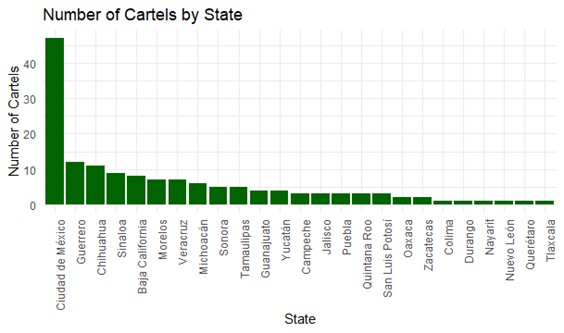
\includegraphics{Figures/Figure1.jpg}

}

\caption{Number of cartels per state}

\end{figure}%%
\begin{figure}[H]

{\centering 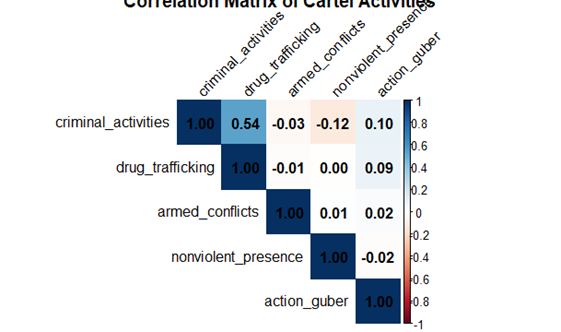
\includegraphics{Figures/Figure2.png}

}

\caption{Correlation matrix of cartel unlawful activities}

\end{figure}%

\section{Research Rationale}\label{research-rationale}

The ERGM is specifically useful in our case as it can lead to a better
understanding of the complex relationships between Mexican cartels and
their rivalries. Our first reason for choosing this model was because of
the network modeling. The research questions that this paper addresses
include the possibility of triadic closures in the network. Those are
especially taken into account by ERGM and are beneficial for our study.
The paper dives deeper into the ERGM terms used in the Results section.
If traditional statistical methods were to be used, it could assume
independence between the observations, and this is not our goal.
Moreover, our hypotheses also could not be tested without the use of
ERGM and based on that could not be supported or rejected. To make sure
everything is correctly set up, we had to include specific terms into
our model to test the hypotheses about the network formation. Another
benefit of ERGM is that it is also flexible to some extent. It can
include the node-level and edge-level attributes. By putting them
together, the model can examine how these factors influence the
formation of network. Last but not least, it also proposes interpretable
coefficients that help us measure the network characteristics, such as
the influence of alliances on rivalry creation. For our ERGM to provide
the best results, we have chosen those terms:

\begin{longtable}[]{@{}
  >{\raggedright\arraybackslash}p{(\columnwidth - 2\tabcolsep) * \real{0.5000}}
  >{\raggedright\arraybackslash}p{(\columnwidth - 2\tabcolsep) * \real{0.5000}}@{}}
\toprule\noalign{}
\begin{minipage}[b]{\linewidth}\raggedright
Term
\end{minipage} & \begin{minipage}[b]{\linewidth}\raggedright
Description
\end{minipage} \\
\midrule\noalign{}
\endhead
\bottomrule\noalign{}
\endlastfoot
edges & Baseline term modeling the likelihood of a rivalry tie forming
between nodes, independent of other factors. \\
gwesp & Models triadic closure by examining the probability of ties
forming in triangles (triadic configurations). It was used as a control
variable to test whether rivalries are more likely to form in triadic
configurations. \\
gwdsp & Models shared enemies by checking if two nodes share a common
enemy, reducing the likelihood of a direct tie between them. \\
degree & A control variable modeling nodes with a specific number of
connections (e.g., nodes with degree = 1). It helps account for
peripheral nodes that might have unique interaction patterns. \\
edgecov & Incorporates the influence of external covariates from a
secondary matrix on tie formation (e.g., state matrices indicating
whether cartels operate in the same states). \\
nodecov & Measures the effect of node-specific attributes (covariates)
on tie formation. Examples include: the number of states a cartel is
active in rivalry network, alliance eigenvector centrality from the
alliances network, and alliance degree from the alliances network. \\
\end{longtable}

Based on our research, there are other methods that would be also
suitable to use in our study. One of them includes stochastic black
models (SBM) or traditional social network analysis (SNA) techniques.
The former would be useful to identify clusters and structures among
network, however, would not provide many interesting insights about
triadic closures or specific network configurations. The latter might
provide additional insights into the descriptive analysis of the network
but, as the goal is to find the interdependence between variables in the
network, it would not be a suitable choice. For that reason, our ERGM is
designed to capture the dependencies as stated in the research questions
and hypotheses. By using the above-mentioned terms and especially
'gwesp', we can observe and find the triadic closures within our model.

\section{Results}\label{results}

This study focuses on cartel rivalry and alliance networks in Mexico. We
calculated the attributes of the alliance network, such as alliance
degree and eigenvector centrality, and used them as exogenous variables
to match with the rival network. In addition, the relationships between
the states based on the cartel were encoded and State Dependency
Matrices were constructed. This report uses ERGM to simulate the
presence of edges in a competitive network as an endogenous network
structure and an exogenous covariate. To address the research questions
and test the hypotheses, ERGMs containing Edges, gwesp, Node Covariates,
Edge Covariates, Degree Distribution, and gwdsp were included.

Gwesp captures triangular closure through weighted statistics. Kstar and
gwdsp measure shared neighbors to reflect clustering effects. Node
covariables like eigenvector centrality and num\_states introduce
heterogeneity. Edge covariates like state dependency matrices encode
geographic dependencies, ensuring the model captures both structural and
contextual dynamics effectively.

\subsection{Data Manipulation}\label{data-manipulation}

First of all, there are Rivalry data, Alliance data, and State
Dependency data in the data source. By filtering the edges of type
Rivalry and Alliance from the original data, we could generate the
Rivalry Network and Alliance Network respectively. In the Rivalry
Network, the study removed all isolated nodes with a degree of 0, which
retains only the cartels involved in competitive relationships.

The data was cleaned, aggregating cartels that had the same name across
multiple rows in the raw dataset into single entities to prepare the
data for analysis. This ensured that every cartel was a unique node,
with their alliances and rivalries, as well as operational attributes,
consolidated in a manner representative of reality. The degree and
influence of each node in the Alliance Network were calculated and added
as node attributes in the Rivalry Network. The number of states for
which each cartel is an active state has been counted and added as an
attribute of the node (as another proxy for geographic extensiveness of
operation of the cartel).

The paper produces two state dependency matrices. One is the binary
matrix, ``state\_dependency\_matrix1'', and one weighted,
``state\_dependency\_matrix2''. The ``state\_dependency\_matrix1''
provides for each pair of cartels if they are or not present in the same
state; while ``state\_dependency\_matrix2'' accounts for the number of
shared states between the pairs. Lastly, the network was transformed
into an object that could be used by ERGM for analysis to fit into the
ERGM framework. NA values were checked and verified that indeed all
attributes that needed validation were correctly assigned to the Rivalry
Network.

\subsection{Modeling Strategy}\label{modeling-strategy}

Our modeling strategy incorporated structural network terms and
covariates to explore the rivalry ties among Mexican cartels. By
iteratively adding and removing terms, this study aimed to balance model
fit, interpretability, and alignment with research questions and
hypotheses.

This study began with a baseline model that included only the edges
term, which represents the baseline likelihood of rivalry edge forming.
This initial model confirmed the sparsity of the network, with a
negative and significant edges coefficient (-5.76, p \textless{} 0.001).
However, this model had poor fit metrics indicating that it did not
capture much of the network's structure. This motivated us to explore
additional terms.

To investigate whether clustering tendencies influenced rivalry
formation, we added the gwesp term with a scaling factor of 0.5. The
inclusion of gwesp slightly improved the AIC (481.23), but the term
itself was not statistically significant. This result indicated that
clustering did not strongly influence rivalry edge in this network,
leading us to delete it in later models.

To measure the impact of the number of cartel connections on rival
relations in the alliance network, this study uses alliance\_degree as a
node attribute. This helps to explore whether the number of alliance
relationships affects the formation of rival relationships. To address
the geographic dynamics of rivalry formation, this research introduced
the ``state\_dependency\_matrix1'' which is the binary matrix for the
active state. The coefficient for this term was highly significant
(3.53, p \textless{} 0.001), showing a strong relationship between
geographic overlap and rivalry formation. The inclusion of this term
drastically improved model fit, reducing the residual deviance and
demonstrating that shared state activity was an important driver of
rivalry ties. However, the strong influence of
``state\_dependency\_matrix1'' increased potential over-reliance on this
single binary covariate. To ensure that the model did not rely on this
term, we conducted similarity analyses. To ensure that the model did not
rely on this term, we conducted similarity analyses. Jaccard similarity
(0.169) and normalized Hamming distance (0.158) calculations revealed
that while the rivalry network and state matrix overlapped to some
extent, the binary matrix explained only part of the network structure.
To optimize the geographical covariates, we used a weighted state
dependency matrix (``state\_dependency\_matrix2'').

The node-level covariates incorporated to address hypotheses related to
cartel centrality. The nodecov(``alliance\_degree'') term, which
measures the direct connections of a cartel in the alliance network,
consistently showed a positive and significant relationship with rivalry
edge (e.g., 0.06, p \textless{} 0.01). On the other hand, the
nodecov(``alliance\_eigenvector'') term, which captures broader
influence in the alliance network, quantifies the influence of cartels
in the alliance network, thereby revealing whether cartels with
significant influence in the alliance network are more likely to form
more rivalries. However, it was not consistently significant, suggesting
that direct connections played a more prominent role than overall
centrality. To address the structural dynamics of rivalry, we added
terms for indirect ties and shared connections. The gwdsp measures the
influence of indirect ties (paths of length 2). While initially
inconsistent, this term became significant in later models, with a
positive coefficient (0.75, p \textless{} 0.001), showing that indirect
ties influenced rivalry formation when combined with other covariates.
The kstar2 term captures the effect of shared enemies and popularity and
it is consistently significant negative coefficient (e.g., -0.84, p
\textless{} 0.001). Finally, the degree1 term, representing peripheral
cartels with only one connection, was positive and significant (1.47, p
\textless{} 0.001), indicating distinct patterns among these cartels in
rivalry formation. This term was included as a control variable to
account for the influence of low-degree nodes on the network structure.

After evaluating all models, Model 9 is the final model. Model 9
integrates findings from previous iterations and explicitly addresses
all research questions and hypotheses. It includes edges, gwdsp, kstar2,
degree1, nodecov(``alliance\_degree''), nodecov(``num\_states''), and
``state\_dependency\_matrix2''. It achieved the best AIC (463.84) and
comparable BIC (510.39).

\subsection{Model Evaluation}\label{model-evaluation}

In conclusion, Model 9 was chosen because it provided the best balance
of fit, interpretability, and alignment with the theoretical framework.
Its inclusion of significant structural and covariate terms ensured a
robust explanation of rivalry formation without over-relying on any
single factor.

\subsubsection{1. MCMC Diagnosis}\label{mcmc-diagnosis}

All the trace plots oscillate steadily around the mean value, indicating
that model have converged and is effectively sampling. No significant
deviations or shifts were found in the graph, so the model is stable,
and the parameters have been selected appropriately. The density plot of
the three terms is smooth and close to normal, indicating that the three
terms performed well in sampling. The goodness of fit for most
parameters is distributed around the median, indicating a good model fit
(Hunter, Goodreau, and Handcock (2008)). The model statistics indicate
that the model can well reproduce the term characteristics of the actual
network. In the node degree distribution graph, the distribution of the
simulated network roughly matches the distribution of the actual
network. In the real network, the degrees of most nodes are concentrated
in a small range (0 to 2), and as the degree increases, the proportion
of nodes decreases rapidly.

The geodesic distance map reveals that the distribution of the simulated
network is consistent with the actual network. However, there is a
deviation in the distribution of nodes with a path length greater than
7.

\subsubsection{2. Model Analysis}\label{model-analysis}

According to Figure 4, the estimated value of edges is -3.69 and the
p-value is less than 0.001, which means that after many iterations, the
network is still very sparse. The edge term describes the overall
tendency of rivalry ties to form, independent of other structural or
covariate terms. Its negative coefficient suggests that rivalry
relationships are generally unlikely to form in the network. These
conflicts do not happen randomly and instead require the influence of
other structural patterns or covariates.

Gwdsp coefficient of 0.621 indicates a strong clustering effect. The low
standard error of 0.178 also confirms its reliability. This high
positive coefficient indicates that the nodes play an important role in
the network structure by sharing indirect connections formed by enemies.
Agglomeration effects show that rivalry networks may be driven by common
enemies, forming more complex indirect interactions rather than a single
direct conflict.

The nodecov.alliance\_eigenvector has a large standard error and
p-values of 0.95 and 0.75 respectively. This indicates that centrality
has no significant impact on network structure and that the indicators
are not estimated accurately. A high p-value is not statistically
significant, so the centrality of the coalition network does not
necessarily make the cartel more likely to be a competitor. The
coefficient (0.076) of nodecov.alliance\_degree is positive, and the
p-value is less than 0.05. This indicates that the number of alliance
relationships is positively correlated with the formation of rivalry
relationships and is significant. The coefficient of kstar is -0.76, and
it has low standard error and p-value. This indicates that the network
does not form a multi-party rivalry structure, and it is more inclined
to a hierarchical structure.

The coefficient for nodecov(num\_states) is -0.004. A smaller negative
coefficient indicates that nodes that are active in more states are
slightly less likely to form a connection. However, the p-value of 0.96
indicates the number of states will not relate to rivalry formation. As
a result, the number of states in which a cartel is active does not have
a meaningful impact on its likelihood to engage in rivalry relationships
within the network. The coefficient of
edgecov(state\_dependency\_matrix2) is 2.4 and p-value is smaller than
0.001. This positive and significant correlation means that geographical
proximity or overlap is a key factor in the formation of rivalry.
Cartels active in the same state are also more likely to conflict,
possibly due to direct competition for territory, markets or resources.

\subsubsection{3. Hypotheses Validation}\label{hypotheses-validation}

To sum up, hypotheses can be verified one by one:

Hypothesis 1 of the RQ1 can be verified using gwdsp and kstar. A
positive coefficient for gwdsp indicates that cartels with a common
enemy tend to avoid and reduce competition. Furthermore, the fact that
kstar has a negative coefficient means that the cartel will not be
connected to another one through indirect links (common enemy).
Therefore, the hypothesis is supported.

In the RQ2, the coefficient for nodecov.alliance\_eigenvector is
statistically insignificant, indicating that the centrality of the
alliance network does not significantly influence the formation of
rivalry. This means that cartels with higher or lower alliance
centrality are not more or less likely to engage in conflicts. Thus,
Hypotheses 1 is rejected. The positive correlation significance of
nodecov.alliance\_degree indicates that cartels with a higher number of
alliance members are more likely to form rival relationships. Therefore,
hypothesis 2 is verified. The negative coefficient for kstar suggests
that cartels avoid conflicts involving multiple parties, even in dense
subnetworks. This indicated the hypothesis that cartels with popularity
(measured by Kstar) are more likely to engage in multi-party conflicts.
As a result, Hypothesis 3 was also rejected.

The result of ``nodecov.num\_states'' in RQ 3, shows that cross-states
alliances will not affect rival relationships, which leads to the
rejection of Hypothesis 1. Hypothesis 2 is confirmed by the large
positive coefficient of ``edgecov.state\_dependency\_matrix''. Cartels
within the same state are more likely to compete due to direct
competition for territory, markets, and resources.

\section{Conclusion}\label{conclusion}

The study focused on the understanding of the rivalry connections
between Mexican cartels using the ERGM. The main research questions that
was addressed, aimed to provide actionable insights into the rivalries
connections between cartels and what influence them. From our analyses,
we gained handful of important insights.

Firstly, for the RQ1, we found a support for the Hypothesis 1. This
means that if two cartels have the same enemy, they are less likely to
form rivalry with each other. The significance came from the positive
coefficient of `gwdsp' term and negative coefficient of the `kstar2'.
Secondly, the hypotheses for RQ2 were rejected. Cartels with higher
centrality measure were not engaged to the higher level in rivalries
with other cartels. This implies that if the cartel has alliance with
higher number of other cartels, it also tends to have more rivals. The
third research question and underling hypotheses were significant and
supported, showing that regions where cartels operate play a crucial
role in the fact that cartels which operate on the same territory become
rivals.

Our findings benefit mostly the policymakers and law enforcement
agencies in Mexico. The case could be also applied to other parts pf the
world, as it provides practical insights into the connections within
crime-focused organizations networks. Based on the geographic insights,
the law enforcement can better allocate the resources to predict the
future possible rivalries and act before they escalate. Moreover, the
researchers would be also beneficiaries of the findings, as it can give
deeper knowledge into the contextual and structural elements influencing
the cartels' behavior.

The open problem that still remains is connected with the incompleteness
of data and/or possible biased information in the analyzed dataset. The
cartels' behavior in terms of rivalries and alliances can also be
influenced by other socio-economic and political factors. Future
research could address those limitations by gathering more data to
ensure and understand the wider perspective on the cartels' behavior.
Next to that, the usage of dynamic ERGMs would also be beneficial for
the research, to capture the potential changes over time.

\section{Appendices}\label{appendices}

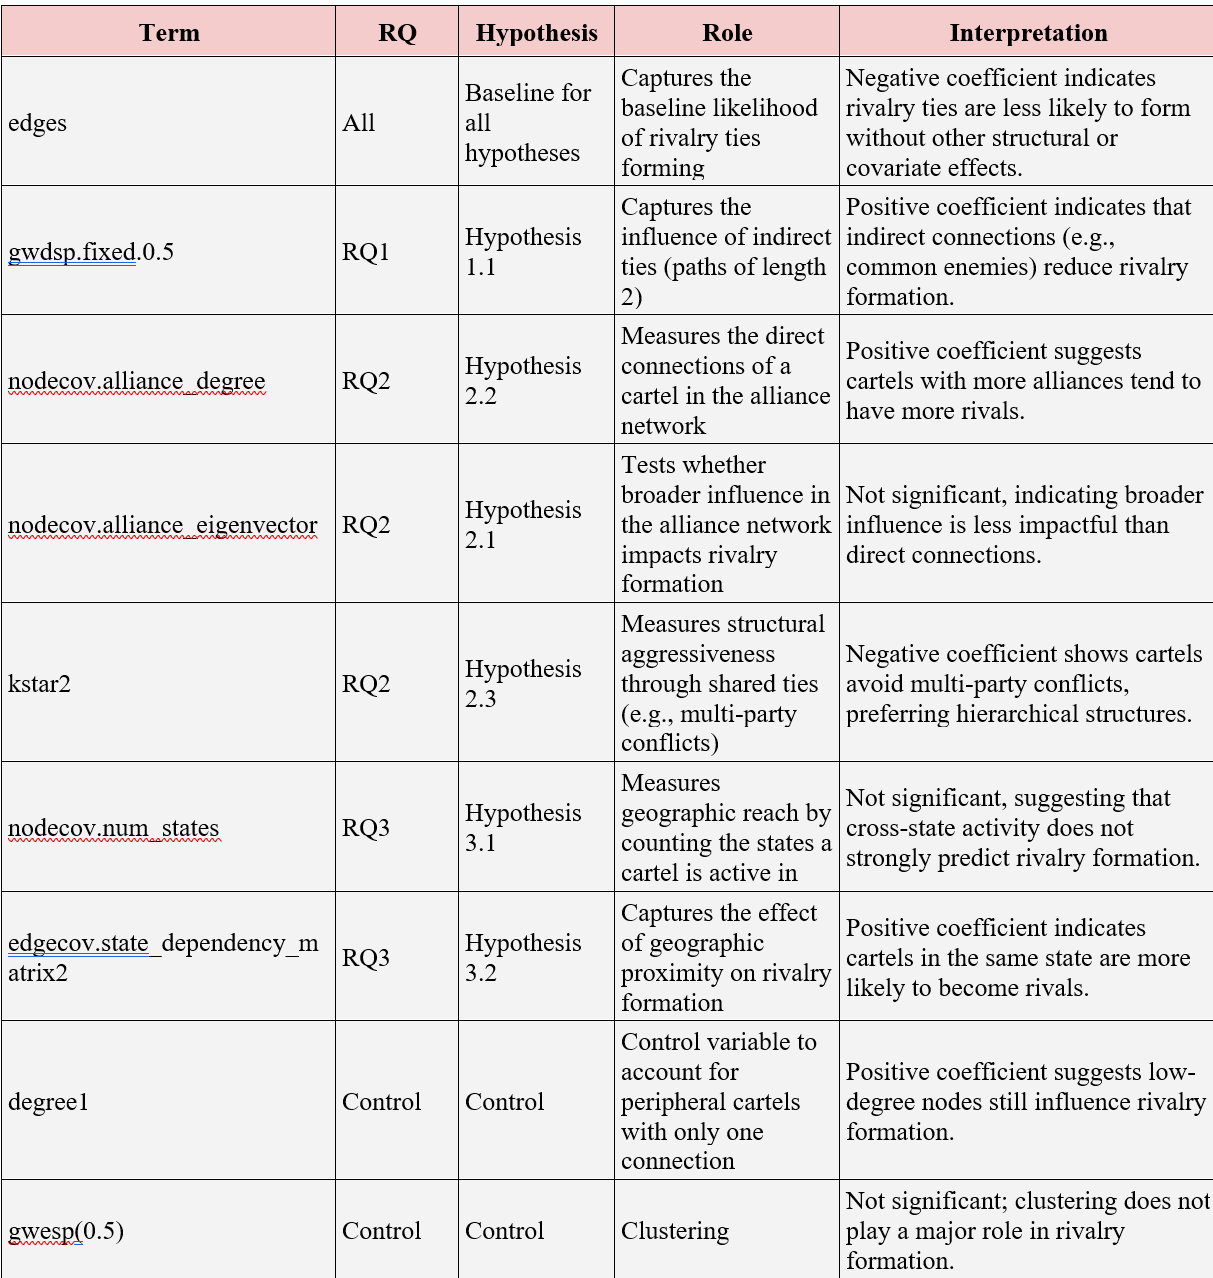
\includegraphics{Figures/Table2.png}

\phantomsection\label{refs}
\begin{CSLReferences}{1}{0}
\bibitem[\citeproctext]{ref-asal2015with}
Asal, Victor H., Hyun Hee Park, R. Karl Rethemeyer, and Gary Ackerman.
2015. {``With Friends Like These . . . Why Terrorist Organizations
Ally.''} \emph{International Public Management Journal} 19 (1): 1--30.
\url{https://doi.org/10.1080/10967494.2015.1027431}.

\bibitem[\citeproctext]{ref-ppdata2020}
CentroGeo - GeoInt. 2020. {``Plataforma de Proyección de Datos Abiertos
(PPData).''} \url{https://ppdata.politicadedrogas.org/\#ppd.gc}.

\bibitem[\citeproctext]{ref-coutinho2020multilevel}
Coutinho, Jorge A., Tomáš Diviák, David Bright, and Johan Koskinen.
2020. {``Multilevel Determinants of Collaboration Between Organised
Criminal Groups.''} \emph{Social Networks} 63: 56--69.
\url{https://doi.org/10.1016/j.socnet.2020.04.002}.

\bibitem[\citeproctext]{ref-dulin2020mexican}
Dulin, Adam L., and Jorge Patiño. 2020. {``Mexican Cartel Expansion: A
Quantitative Examination of Factors Associated with Territorial
Claims.''} \emph{Crime, Law and Social Change} 73: 315--36.

\bibitem[\citeproctext]{ref-europolDEAcomplexities}
Europol-DEA, European Monitoring Centre for Drugs, Drug Addiction,
Beltrán Leyva Organisation, Sinaloa Cartel, Jalisco New Generation
Cartel, United States Drug Enforcement Administration, et al. n.d.
{``Complexities and Conveniences in the International Drug Trade: The
Involvement of Mexican Criminal Actors in the EU Drug Market.''}
Europol-DEA Public Document.

\bibitem[\citeproctext]{ref-hunter2008goodness}
Hunter, David R., Steven M. Goodreau, and Mark S. Handcock. 2008.
{``Goodness of Fit of Social Network Models.''} \emph{Journal of the
American Statistical Association} 103 (481): 248--58.
\url{https://doi.org/10.1198/016214507000000446}.

\bibitem[\citeproctext]{ref-jones2022social}
Jones, Nathan P., Ioana A. Chindea, Daniel W. Argomedo, and John P.
Sullivan. 2022. {``A Social Network Analysis of Mexico's Dark Network
Alliance Structure.''} \emph{Journal of Strategic Security} 15 (4):
76--105.

\bibitem[\citeproctext]{ref-nix2016use}
Nix, Justin, Michael R. Smith, Matthew Petrocelli, Jeff Rojek, and
Victor M. Manjarrez. 2016. {``The Use of Social Media by Alleged Members
of Mexican Cartels and Affiliated Drug Trafficking Organizations.''}
\emph{Journal of Homeland Security and Emergency Management} 13 (3):
395--418. \url{https://doi.org/10.1515/jhsem-2015-0084}.

\bibitem[\citeproctext]{ref-smith2021dope}
Smith, Benjamin T. 2021. \emph{The Dope: The Real History of the Mexican
Drug Trade}. Random House.

\bibitem[\citeproctext]{ref-staff2022social}
Staff, Small Wars Journal. n.d. {``A Social Network Analysis of Genaro
García Luna and His Alleged Ties to the Sinaloa Cartel.''} Small Wars
Journal by Arizona State University.

\bibitem[\citeproctext]{ref-trejo2018why}
Trejo, Guillermo, and Sandra Ley. 2018. {``Why Did Drug Cartels Go to
War in Mexico? Subnational Party Alternation, the Breakdown of Criminal
Protection, and the Onset of Large-Scale Violence.''} \emph{Comparative
Political Studies} 51 (7): 900--937.

\bibitem[\citeproctext]{ref-ucdp}
Uppsala Conflict Data Program, UCDP -. 2022. {``UCDP - Uppsala Conflict
Data Program.''}

\end{CSLReferences}




\end{document}
